\documentclass[9pt,twocolumn,twoside]{gsajnl}
% Use the documentclass option 'lineno' to view line numbers

\articletype{inv} % article type
% {inv} Investigation
% {gs} Genomic Selection
% {goi} Genetics of Immunity
% {gos} Genetics of Sex
% {mp} Multiparental Populations


\title{Prostate Adenocarcinoma insights: Gene Expression approach from TCGA RNA-seq data}

\author[$\ast$,$\dagger$]{Adria Auladell-Martin}
\author[$\ast$,$\dagger$]{Joan Marti-Carreras}
\author[$\ast$,$\dagger$]{David Mas-Ponte}
\author[$\ast$,1]{Robert Castelo-Valdueza}

\affil[$\ast$]{M.Sc. in Bioinformatics at Department of Experimental and Health Sciences (CEXS), Universitat Pompeu Fabra}
\affil[$\dagger$]{Authors Contributed Equally to this work}

\keywords{prostate cancer; adenocarcinoma; RNA-Seq; paired data.}

\runningtitle{GENETICS} % For use in the footer

\correspondingauthor{Auladell-Martin}

\begin{abstract}
The abstract should be written for people who may not read the entire paper, so it must stand on its own. The impression it makes usually determines whether the reader will go on to read the article, so the abstract must be engaging, clear, and concise. In addition, the abstract may be the only part of the article that is indexed in databases, so it must accurately reflect the content of the article. A well-written abstract is the  most effective way to reach intended readers, leading to more robust search, retrieval, and usage of the article.

\textcolor{red}{--------}

Transciptomics studies have improved substantially the molecular analysis of cancer, with the discovery of many new drug targets. The Cancer Genome Atlas Project has provided to the research society high quality RNA-seq data in many different tumour types. Prostate cancer, or prostate adenocarcinoma, is the second most deadly cancer disease, and one with the highest prevalences. The present article aims to perform an analysis of the differential expression and a functional analysis of rna seq data obtained from The Cancer Genome Atlas project. With previous subsetting and normalization, a paired design of 42 tumor and 42 normal samples was used. Differential expression analysis was realized by multiple linear regression. Finally, a functional analysis was realized by hypergeometric test on gene ontology and gene set enrichment analysis/gene set variation analysis on various pathway datasets. \textcolor{red}{falten els resultats conclus ojo}

\end{abstract}

\setboolean{displaycopyright}{true}

\begin{document}

\maketitle
\thispagestyle{firststyle}
\marginmark
\firstpagefootnote
\correspondingauthoraffiliation{adria.auladell@estudiant.upf.edu, joan.marti02@estudiant.upf.edu, david.mas@estudiant.upf.edu. Corresponding author: Robert Castelo Valdueza, robert.castelo@upf.edu.}
\vspace{-11pt}%

\lettrine[lines=2]{\color{color2}T}{}his \textit{Genetics} journal template is provided to help you write your work in the correct journal format. Instructions for use are provided below.

\section*{Your Abstract}

In addition to the guidelines provided in the example abstract above, your abstract should:

\begin{itemize}
\item provide a synopsis of the entire article;
\item begin with the broad context of the study, followed by specific background for the study;
\item describe the purpose, methods and procedures, core findings and results, and conclusions of the study;
\item emphasize new or important aspects of the research;
\item engage the broad readership of GENETICS and be understandable to a diverse audience (avoid using jargon);
\item be a single paragraph of less than 250 words;
\item contain the full name of the organism studied;
\item NOT contain citations or abbreviations.
\end{itemize}


\section*{Introduction}

Prostate adenocarcinoma (PRAC), also referred as prostate cancer, is  the second most deadly cancer disease (following lung cancer), and one with the highest prevalences. As the American Cancer Society explains, about 1 man in 7 will be diagnosed with PRAC during his lifespan, and of those diagnosed about 60\% are men over 65 years. Despite it might affect younger men (under 40 years old), it is not frequent. The mean of diagnosis is around 66 years old \cite{prostatestatistics}.

For patients whose cancer has spread, their survival time is usually one to three years. It was estimated that for 2011, 240,890 men would be diagnosed and 33,720 would die from prostate cancer.


Since the first publication of the human genome, multiple international projects have been carried in order to study the genetic bases of the this pathology. One of the most prominent is The Cancer Genome Atlas Project (TCGA) \cite{tgca}. Recently, part of its information was released with part of the original data \cite{Rahman15112015}. TCGA established the following points:

\begin{itemize}
\item 74\% of all tumors being assignable to one of seven molecular classes based on distinct oncogenes drivers:
        fusions involving (1) ERG, (2) ETV1, (3) ETV4, or (4) FLI1 (46\%, 8\%, 4\%, and 1\%, respectively)
        mutations in (5) SPOP or (6) FOXA1; or (7) IDH1. (11\%, 3\%, and 1\%, respectively).
\item 25\% of the prostate cancers had a presumed actionable lesion in the PI3K or MAPK signalling pathways, and DNA repair genes were inactivated in 19\%.
\end{itemize}


The aim of this study is to provide a second outlook to the released data of the TCGA. For doing so we are to perform a differential expression analysis using paired data from the TCGA.

\section*{Materials and Methods}



The examination of the RNA counts can be performed in an average laptop. As a limiting factor for analysing the data, it is recommended to have at least 4 Gb of RAM and CPU Intel Core i5 or superior. HDD memory is not a limiting factor for this analysis.

\begin{figure*}[!h]
\centering
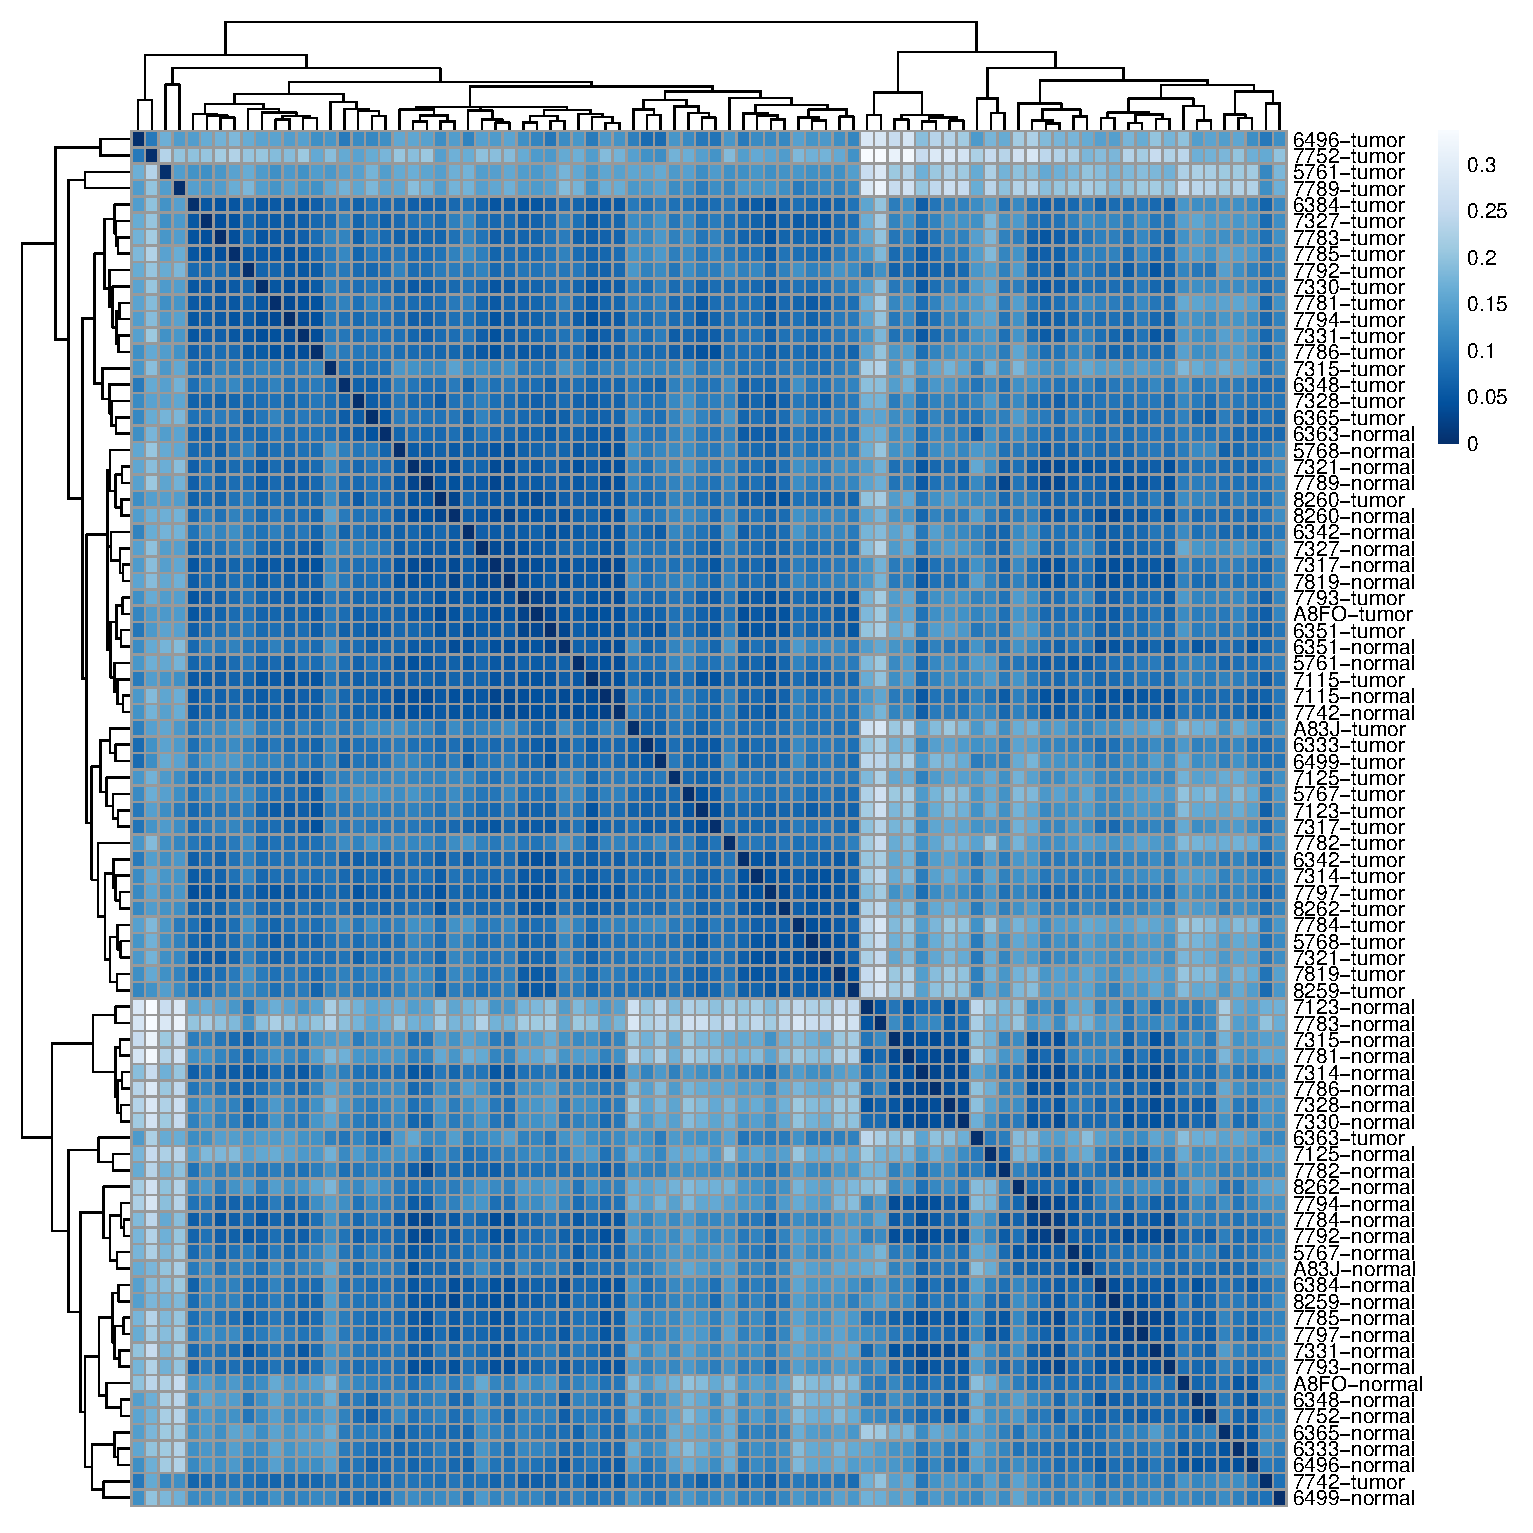
\includegraphics[width=\textwidth]{Clustering.eps}
\caption{Initial Cluster of Final data set clustered by gene expression levels. Although some samples are not clustered ideally with their correspondent type, 2 groups can be distinguished clearly. The top-left group contains most of the tumour samples and the bottom-right contains most of the Normal samples.
}
\label{fig:Clustering}
\end{figure*}

The software used was R version 3.3.0 "Supposedly Educational" \cite{R}. Main packages where download and installed through Bioconductor version 3.3 (BiocInstaller 1.22.2)\cite{bioconductor}.

Detailed information about package versions can be found on the section "Session Info" of the Supplementary Materials.

In the following sections we describe briefly our analyses. However, a reproducible version of our analysis with all the code elements is also available in the supplementary material.

\subsection*{Data Availability}

The data sets are tables of RNA-seq counts generated by Rahman et al. \cite{Rahman15112015} from the TCGA raw sequence read data using the Rsubread/featureCounts pipeline for all data sets \cite{Rsubread}. They also processed clinical data that forms part of these data sets. PRAC dataset consist initially of 502 tumour samples and 52 normal samples. The phenotypic variable that indicates the tumour or normal status of the sample is called type.

The data was used for this analysis is a variation of the above mentioned datasets, curated by PhD. Robert Castelo-Valdueza \url{http://functionalgenomics.upf.edu/courses/IEO/projects/datasets/sePRAD.rds}.

\subsection*{Experimental Design}

From the initial dataset, there are 52 normal samples and 502 tumour samples. Searching for coincidences in the patients barcode, it was found out that the dataset had mixed paired and unpaired data. It was decided that the paired design was a better choice, as it takes better into account the differences between subjects.

After applying the corresponding logical mask, the dataset was composed by 50 normal samples and 50 tumour samples.

\subsection*{Quality Assessment and Normalization}

DGE functions were used for normalization, which belongs to edgeR package \cite{Robinson01012010}. Normalization factors were calculated and counts per million reads (logCPM) computed.

LogCPM distributions area compared between normal samples and tumour samples. There are no significant differences. Transcripts with logCPM < 1 were deprecated.

Despite there was a peak of high library size in the library size distribution, it was decided to not to take it out. The rest of the distribution was considered to be uniform.

When plotting the log ratio - mean average plots (MA-plots) for all samples, it was noticed that the normalization procedure succeeded. Any deviation was considered as non-significance.

\subsection*{Batch Effect Identification}

Batch effect was evaluated by means of the TCGA barcode information. The code specified center of analysis, tissue source site and plate of the NGS machine. The center was the University of North Carolina for all samples and the tissue source site/plate variables were equilibrated in the tumour/normal comparison (see SM).

To evaluate possible anomalous samples, hierarchical clustering (HC) from \cite{pheatmap} package and multidimensional scaling (MDS) from \cite{limma} package were performed. HC, clustered by Spearman correlation, presented mainly a good clustering, with some of the paired samples clustering together due to the similarities within individual (see SM). MDS plot presented an anomalous clustering of normal samples from the same batch. These samples were filtered out, remaining 42 tumour and 42 normal samples.



\subsection*{Differential Expression Analysis}

A design matrix was built with sample type (tumor/normal). LogCPM measurements were corrected with the  voom (mean-variance relationship of the log-counts) function present in limma package \cite{voom}. As a covariates,  patient barcode and surrogate variables inferred by SVA analysis were included. Surrogate variables are covariates constructed directly from high-dimensional data that can be used in subsequent analyses to adjust for unknown, unmodeled, or latent sources of noise analysis \cite{GSVA}.

With the design matrix and voom logCPM values, Multiple linear regression (MLR) was performed with \cite{limma} package. From MLR analysis, t statistics, moderated F-statistics and  log-odds ratios were caculated with empirical Bayes statistics from \cite{limma} package. P-values were adjusted with FDR measurements and cutoff was established at genes presenting 1\% of FDR. To evaluate results p-values and moderated t-statistics were plotted and DE genes were visualized in volcano plots and  MA plots  from \cite{limma} package (see SM). Top DE hits were visualized with Gviz package. \textcolor{red}{Creieu que cal aixo final?}


\subsection*{Functional Enrichment}


The resulting DE genes from the previous analyses have been tested for functional enrichment using Gene Ontology gene sets. A hyper-geometrical test from the GOstats package \cite{GOstats} was used. As parameters, a p-value cutoff of 0.01 have been set in order to filter only the most significant results. Then, the results have been pruned again for sets with at least 8 genes to avoid extreme results with infinite OddsRatio.

The same analysis have been also performed in the DE over-expressed and under-expressed gene lists to clarify if the GO biological process is indeed enhanced or decreased in tumor cells. The aim of this stratified analysis is to improve the biological content of our results.


\subsection*{Gene Set Expression Analysis}
In order to analyse differential expression in gene sets and not uniquely at the gene level 2 different approaches have been used, a Gene Set Enrichment Analysis (GSEA) and a Gene Set Variation Analysis (GSVA).


For both GSEA and GSVA the gene sets from the GSVAdata package \cite{GSVAdata} have been selected. After that, the original gene sets were reduced only to curated gene sets  (C2 type) . In this case the KEGG  \cite{kanehisa2016kegg}, Reactome \cite{fabregat2016reactome} and   Biocarta \cite{nishimura2001biocarta} databases were selected. Gene Sets related with Prostate Cancer have been also included from the same data package.


The package GSEABase \cite{GSEABase} was used to define Gene Sets and match gene identifiers to our Entrez Id codes. The classic GSEA consist in the generation of an incidence matrix that let us build a Enrichment Score by that is dependent on how many genes from the gene set are ranked as most DE genes. It is also an enrichment approach, however, it uses the expression values from the expressed genes to rank them so therefore it is been using expression data.

The GSVA package \cite{GSVA} was used to define the set expression values. Then, limma  \cite{limma} and SVA packages were used to perform the linear regression and to improve the model respectively \cite{leek2007capturing,svamanual} . Finally, the 30 top DE pathways have been clustered by sample in order to obtain a clear visualization of the ones over and under-expressed in tumor and normal samples.


\section*{Results}
\subsubsection*{Differential Expression Analysis}

\begin{figure}[!h]
\centering
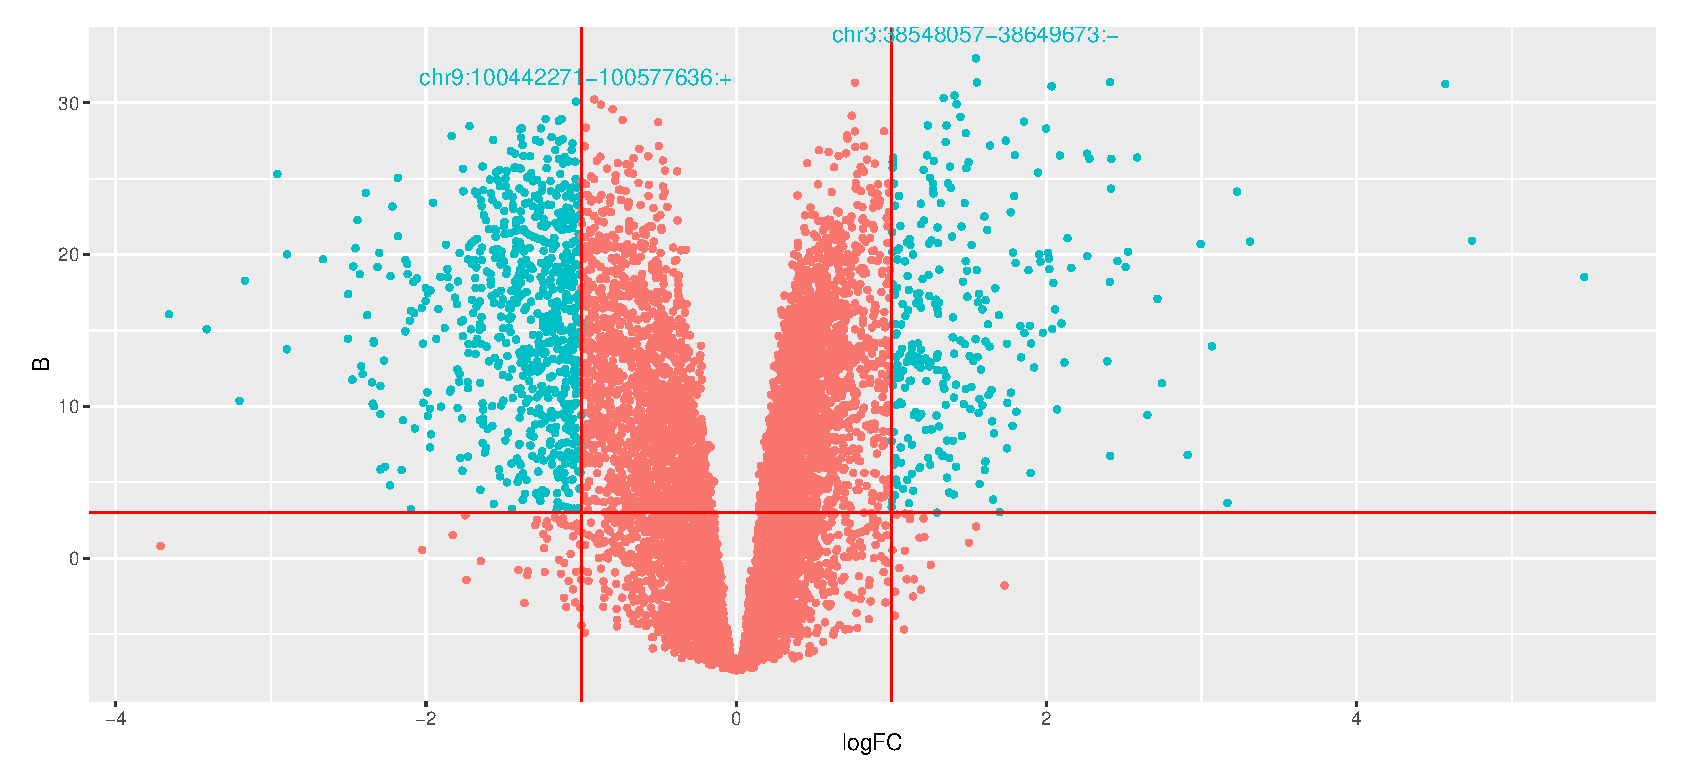
\includegraphics[width=\linewidth]{Volcano.eps}
\caption{Volcano plot of the studies genes. Crossing lines represent the threshold by which genes have been minimally accepted. Most scoring genes are highlighted.
}
\label{fig:volcano}
\end{figure}

After computing the multiple linear model test, and the eBayes test \cite{limma} 	it was found out that:

\begin{itemize}
\item 2168 genes are under-expressed in tumour samples compared to normal samples.
\item 7569 genes have no significant difference in their expression between sample types.
\item 2127 genes are over-expressed in tumour samples compared to normal samples.
\end{itemize}

After defining the null model (bcr patient code variable, which corrects by patients variability) and computing the SV analysis, the volcano plot (\ref{fig:volcano}) was performed to graphically represent the distribution of genes by its B (signification) and its log fold changes (intensity).

Genes out of the area formed by minimum levels of signification (depends on FDR) and minimum intensity (expression is doubled).




Despite that there are lots of genes that fall out of the rejection zones, in fact they conform a gradient of significant gene, only the topmost 5 will be taken into account for the rest of the article, as it is more likely that their values are worth. These 5 genes were then searched using the UCSC browser, using the RefSeq track, as it is more up-to-date.
\begin{itemize}
\item chr1:225 codifies for \href{http://www.genecards.org/cgi-bin/carddisp.pl?gene=EPHA8}{EPHA8} which is an ephrin receptor, a neuronal factor.
\item chr2:101 codifies for \href{http://www.genecards.org/cgi-bin/carddisp.pl?gene=SNORD89}{SNORD89} which is a small nucleolar RNA.
\item chr3:385 codifies for \href{http://www.genecards.org/cgi-bin/carddisp.pl?gene=SCN5A}{SCN5A} which is a sodium channel voltage gated V Type.
\item chr11:11 codifies for \href{http://www.ensembl.org/Homo_sapiens/Gene/Summary?g=ENSG00000255292;r=11:112086903-112193805}{AP002884.2} which seems to mitocondrial protein (but does not appear on RefSeq).
\item chrX:492 codifies \href{http://www.genecards.org/cgi-bin/carddisp.pl?gene=CACNA1F}{CACNA1F} which is a calcium channel voltage dependant L type.
\end{itemize}

EPHA8 is a prognosis marker for cancer (malignant marker). It appears over-expressed in several tumour types, between them prostate cancer \cite{proteinatlas}.

SNORD89 is related with several cancer-related pathways:  anaplastic large cell lymphomas, lymphoma (NHL) cell lines, metastasis and death cell in colon cancer, prostate cancer, ovarian adenocarcinomas, etc \cite{tcng}.

SCN5A is a voltage-gated sodium channel (VGSC), a group that is known to be related with metastatic potential of breast cancer, prostate cancer and lung cancer between others \cite{Nelson2015}.

AP002884.2 seems to be an unmapped transcript. A more accurated display of the region, reveal that AP002884.2 compromises 2 genes SDHD-006 and BCO2-009. SDHD-006 is the 6th subunit of the succinate dehydrogenase, which is known to play a role as oncometabolite \cite{oncometabolites} and BCO2-009 is related with the synthesis of vitamin A through oxidation of carotenoids  and beta-carotene and have and strong relation with all kinds of cancer \cite{proteinatlas}.

We suggest that in the case of AP002884.2 there has been an error in the mapping phase of the reads. We have considered to take into account both proteins (SDHD-006 and BCO2-009) has both can be traced to carcinogenic processes.

CACNA1F is related with several cancer-related pathways: colon cancer, breast cancer, melanoma, myeloma, prostate cancer, etc \cite{tcng}.

It can be concluded, thus, that the main over-expressed genes in tumour samples are those related with signalling, metabolism and transcription modulation; fields that are usually related to carcinogenic processes.

\subsubsection*{Functional Enrichment}

From the 11143 gene ontology (GO) biological processes (BP) terms tested, only 21 presented significant results (p < 0.01). The top 5 results in odds ratio decreasing order are listed in Table \ref{tab:GOenrichment}.

The first result is related with processes that modulate the frequency, rate or extent of astrocyte differentiation (GO:0048710). This result coincides with other studies provided by \cite{neuroendocrine3, neuroendocrine2} and the review realized by \cite{neuroendocrine1}. Some of the set genes haven been described in other studies as neurodifferentiaton markers, such as EPHA4 \cite{neuroendocrine_EPA}, SEPRINE2 \cite{mckee2013protease} and others. 

Response to vitamin A is a unexpected result: it is well known in prostate cancer the relationship with vitamin D \citep{vitamin0,vitamind1,vitamind2,vitamind3}, but little is known of the relationship with vitamin A. \cite{vitamina1} described a correlation between lack of vitamin A and prostate cancer, but there is no much other analysis in such aspect. Also, \cite{vitamina2} studied the relationship between vitamin A and apoptosis in prostate cancer, relating indirectly some of the genes such as retinoic acid receptor-beta (RARA), whose expression could be downregulated in cancer. 

Both icosanoid secretion and fatty acid transport have been related with cancer \citep{fat1,fat2}. Eicosanoid are biological lipid molecules that are implicated in pathological processes. Being part of the  cyclooxygenase (COX) and lipoxygenase (LOX) pathways, they present mediator effect in the proliferation of cancerous cells and regulate tumor vascularization \citep{fatvascu} As we can see, the gene sets are almost identical, with SLCO2A1 present as a difference in fatty acid transport. 

Finally, hystone acetylation (HA) presents relationship with cancer due to the regulatory role during transcription of genes through its influence on chromatin conformation \citep{histoneacet, histoneacet2, histoneacet3, histoneacet4}. Since in GO studies we only evaluate DE gene sets, this gene ontology factor can be related with the normal type. This would coincide with the expectation, since HA supresses tumour formation \cite{histonea}. 


One consideration about the Gene Ontology analysis using hypergeometric tests is the variation of results with the parametic adjustment of the researcher. Pvalue cutoff and minimal gene sizes change the results of the functional enrichment analysis considerably. This makes the assay subjective for each researcher parametic decisions. With that purpose in mind, our analysis was restrictive to an small specific subset of GO terms, losing some other authentic results but reassuring the ones obtained. 

\subsubsection*{Gene set expression analysis}

As mentioned above, 2 approaches have been used to detect Differential Expression at gene set level. The results from the enrichment approach are in table \ref{tab:GSEAenrichment}.

\paragraph{Under-expression of Endogenous Sterols } The genes in this gene set,


Purament el resultat


\section*{Discussion}

Creure'ns o no els resultats

\section*{Figures and Tables}

Figures and Tables should be labelled and referenced in the standard way using the \verb|\label{}| and \verb|\ref{}| commands.



\begin{figure*}[htbp]
\centering
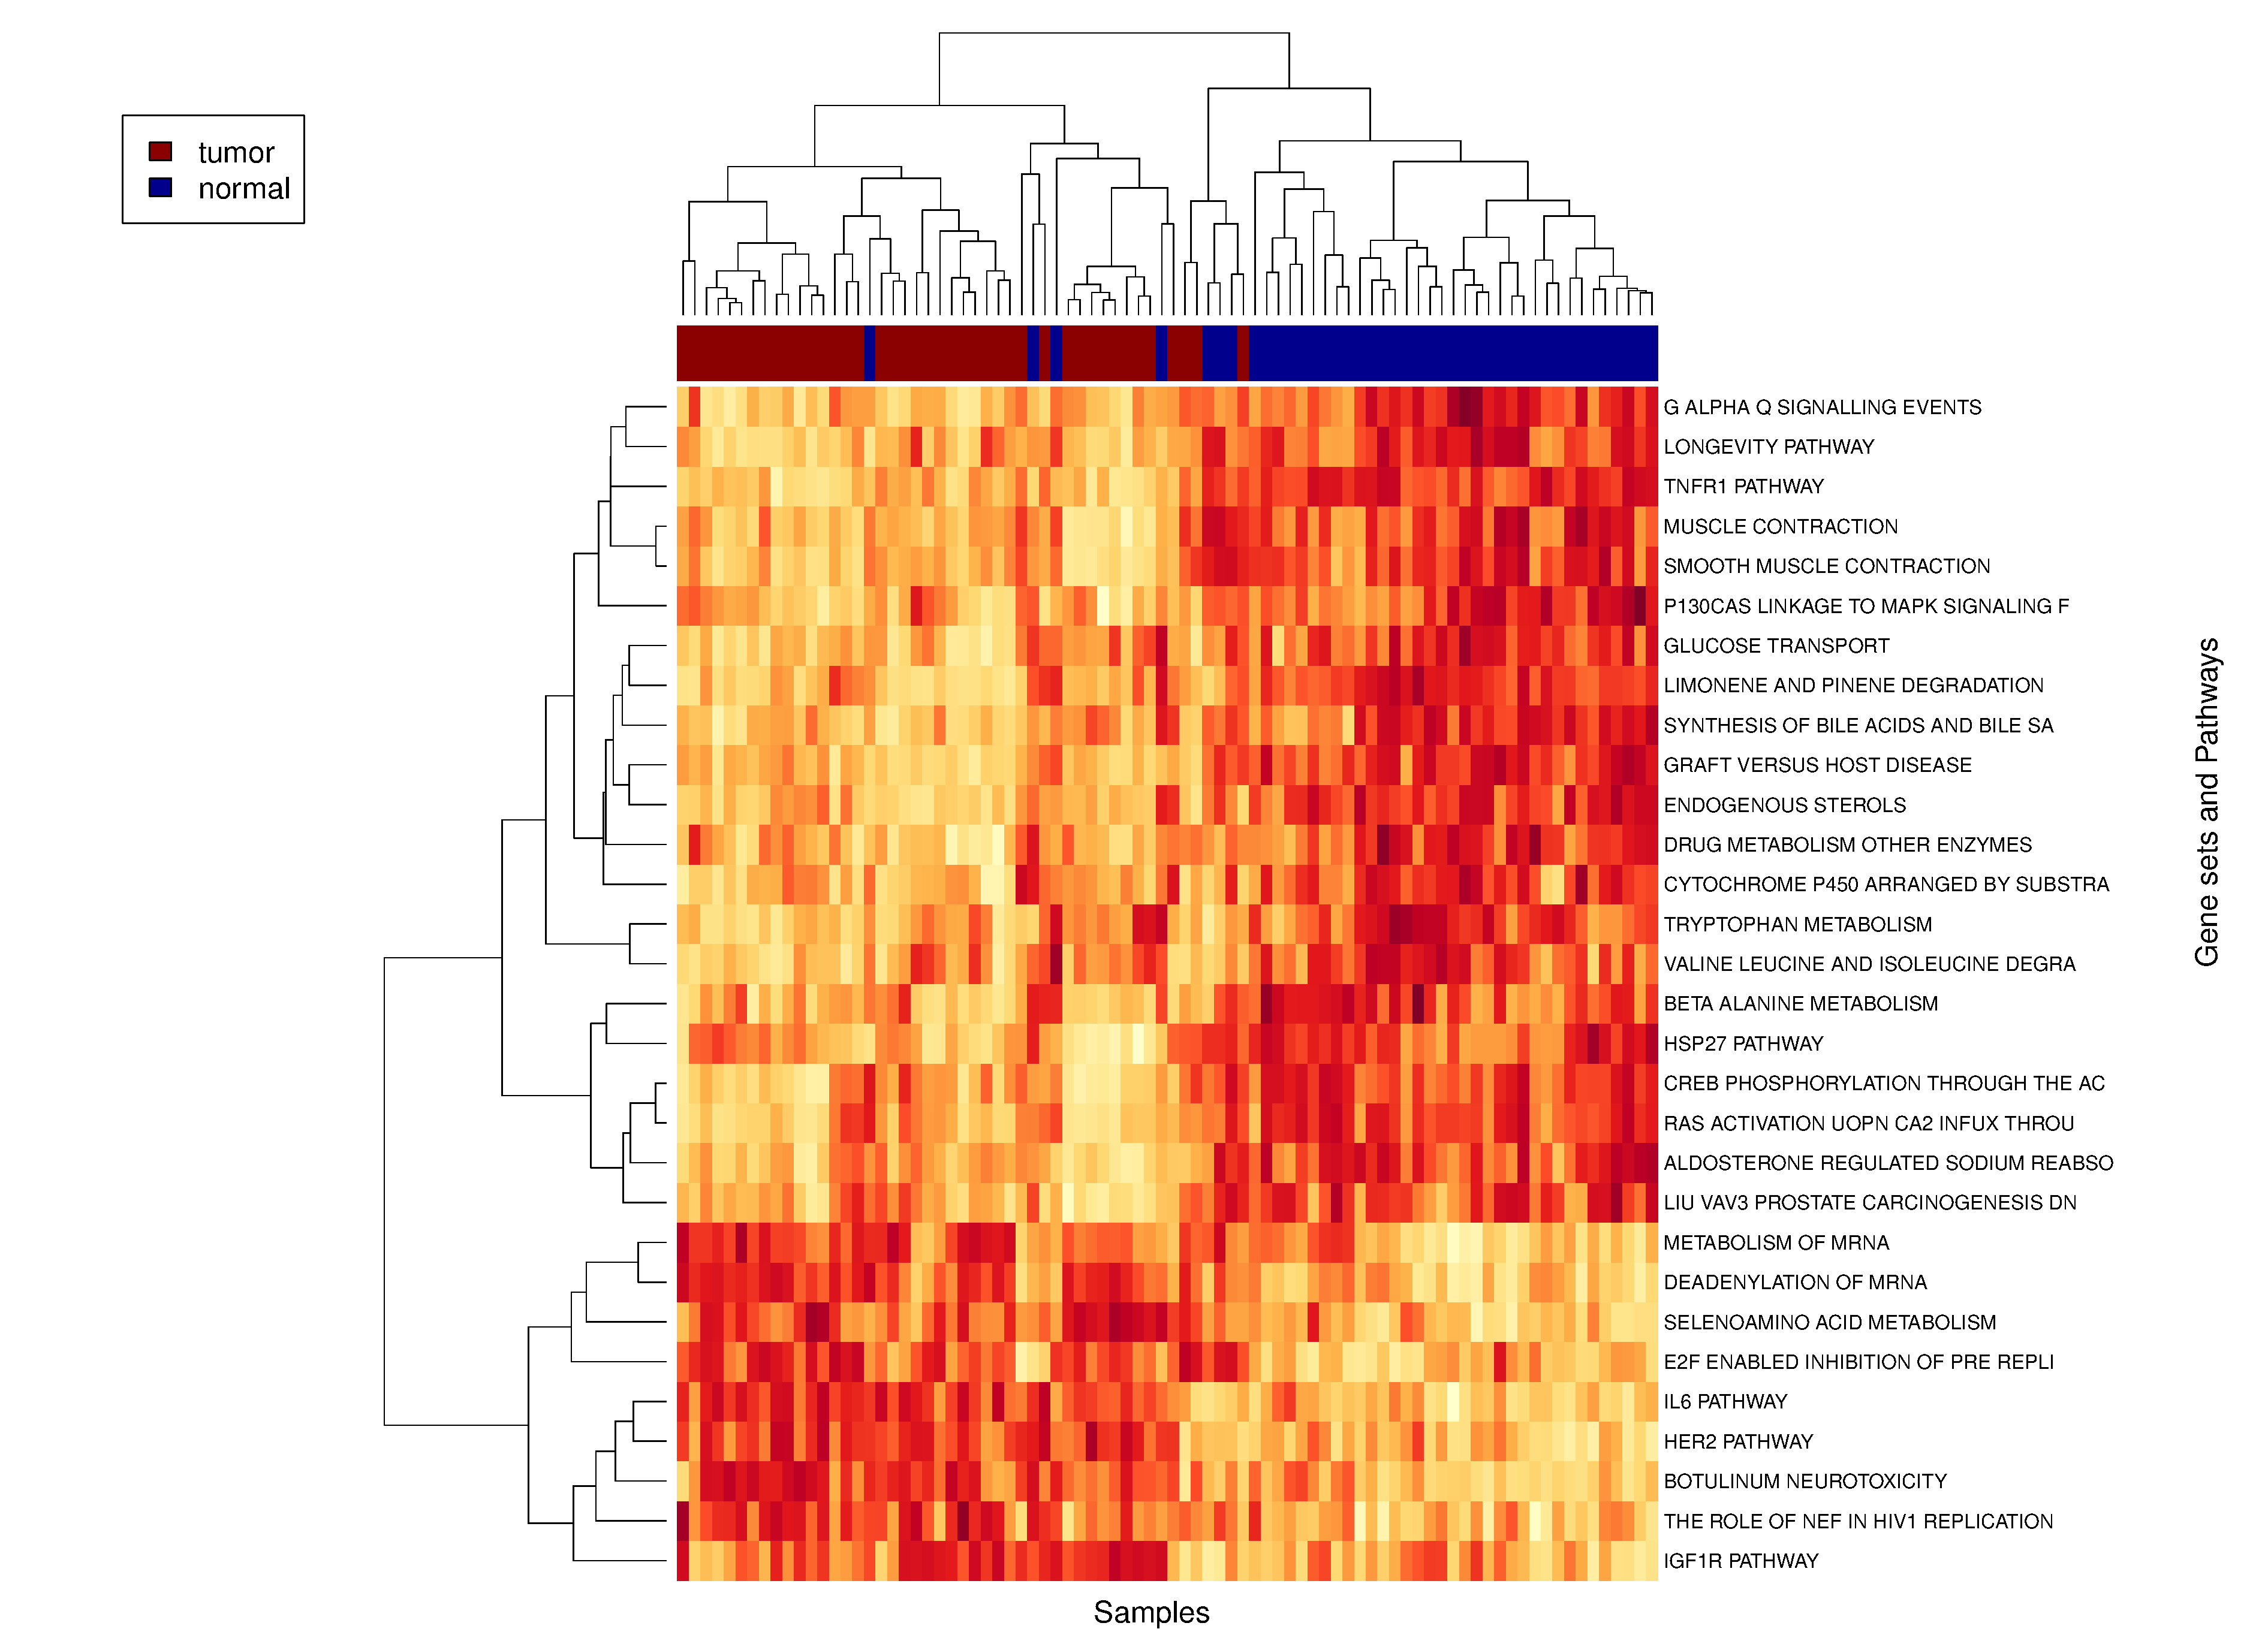
\includegraphics[width=\linewidth]{ClusteringGSVA.eps}
\caption{Heatmap from the Clustering of the DE gene sets obtained from GSVA and samples.
}
\label{fig:ClusteringGSVA}
\end{figure*}




\subsection*{Sample Table}

Table \ref{tab:shape-functions} shows an example table. Avoid shading, color type, line drawings, graphics, or other illustrations within tables. Use tables for data only; present drawings, graphics, and illustrations as separate figures. Histograms should not be used to present data that can be captured easily in text or small tables, as they take up much more space.

Tables numbers are given in Arabic numerals. Tables should not be numbered 1A, 1B, etc., but if necessary, interior parts of the table can be labeled A, B, etc. for easy reference in the text.

% latex table generated in R 3.3.0 by xtable 1.8-2 package
% Tue Jun 14 13:44:38 2016
\begin{table*}[htbp]
\centering
\caption{\bf GO enriched terms}
\begin{tableminipage}{\textwidth}
 \begin{tabular}{|l|c|r|r|r|r|r|p{3cm}|p{4.3cm}|}
  \hline
 & GOBPID & Pvalue & OddsRatio & ExpCount & Count & Size & Term & Genes \\
  \hline
 1 & GO:0048710 & 0.00 & 11.20 & 7.53 &  13 &  14 & regulation of astrocyte differentiation & DAB1, EPHA4, F2, FGFR3, ATF5, PRPF19, BIN1, HES1, IL1B, NTRK3, SERPINE2, CNTN2, NR2E1 \\
   2 & GO:0033189 & 0.01 & 9.47 & 6.45 &  11 &  12 & response to vitamin A & DNMT3A, DNMT3B, GATA4, ARG1, LTC4S, RARA, RXRA, TSHB, TYMS, CAT, ALDH1A2 \\
   3 & GO:0032309 & 0.01 & 6.03 & 8.60 &  14 &  16 & icosanoid secretion & ABCC4, ACE, DRD3, AGTR2, ACSL4, ANXA1, IL1B, NTSR1, OXT, P2RX7, BDKRB2, SYK, CYP4F2, TNFSF11 \\
   4 & GO:1901571 & 0.01 & 4.31 & 9.68 &  15 &  18 & fatty acid derivative transport & ABCC4, ACE, DRD3, AGTR2, ACSL4, ANXA1, IL1B, NTSR1, OXT, P2RX7, BDKRB2, SLCO2A1, SYK, CYP4F2, TNFSF11 \\
   5 & GO:0043966 & 0.01 & 3.45 & 13.45 &  20 &  25 & histone H3 acetylation & TRIM16, TAF6L, WDR5, CHEK1, KAT7, SGF29, DR1, BRD4, KAT6B, WBP2, SIN3A, BRPF3, PER1, PIH1D1, CSRP2BP, BRCA2, TAF10, BRPF1, KAT2B, SUPT7L \\
   \hline
 \end{tabular}
 \label{tab:GOenrichment}
\end{tableminipage}
\end{table*}



\begin{table*}[htbp]
\centering
\caption{\bf GSEA enriched normal scores}
\begin{tableminipage}{\textwidth}
\begin{tabular}{|l|c|c|p{3cm}|}
 \hline
Gene Set & Relative tumor expression &  Z-value & Genes \\
  \hline
REACTOME DEADENYLATION OF MRNA & Over-Expressed  & 19.19 & EIF4A1, EIF4A2, EIF4B, EIF4E, EIF4G1, CNOT2, CNOT4, RQCD1, CNOT8, PAN2, CNOT1, CNOT10, PABPC1, CNOT7, CNOT6, TNKS1BP1, CNOT6L, PAN3 \\
REACTOME SMOOTH MUSCLE CONTRACTION & Under-Expressed & 18.70 & ACTA2, ACTG2, CALM1, CALM3, ITGA1, ITGB5, PXN, TPM2, VCL, SORBS1 \\
REACTOME BOTULINUM NEUROTOXICITY & Over-Expressed &  17.62 & SNAP25, SYT1, STX16, STX11, STX10, STX6, STX12, STX1B \\
REACTOME ENDOGENOUS STEROLS & Under-Expressed & 17.54 & CYP8B1, CYP11B1, CYP51A1, CYP46A1, CYP39A1 \\
\hline
\end{tabular}
\label{tab:GSEAenrichment}
\end{tableminipage}
\end{table*}






\bibliography{prac-bibliography}

\end{document}
